%+TITLE: Mecánica clásica
%+DESCRIPTION: Repaso de los conceptos escenciales de la mecánica clásica que necesitaremos
\documentclass[11pt,a4paper]{article}

\usepackage[utf8]{inputenc}
\usepackage[T1]{fontenc}
\usepackage[spanish,es-nodecimaldot]{babel}
\usepackage{lmodern}
\usepackage{amsmath,amssymb,mathtools}
\usepackage{graphicx}
\usepackage{xcolor}
\usepackage{geometry}
\usepackage{enumitem}
\usepackage{microtype}

\geometry{margin=2.3cm}
\setlength{\parindent}{0pt}
\setlength{\parskip}{0.65em}
\setlist[itemize]{leftmargin=1.6em,itemsep=0.25em,topsep=0.25em}

\definecolor{title-red}{RGB}{165,25,20}
\definecolor{concept-green}{RGB}{20,125,45}
\newcommand{\concept}[1]{\textcolor{concept-green}{#1}}

\newcommand{\ket}[1]{\left|#1\right\rangle}
\newcommand{\bra}[1]{\left\langle#1\right|}
\newcommand{\braket}[2]{\left\langle #1\middle|#2\right\rangle}
\newcommand{\hc}{\mathrm{h.c.}}
\newcommand{\Tr}{\operatorname{Tr}}
\newcommand{\Diffs}{\mathrm{Diffs}}

\begin{document}

Queremos describir la dinámica general de un sistema. Para eso necesitamos identificar las variables que lo describen (posiciones de los centros de masa, ángulos de los cuerpos rígidos, etc.). Estas se llaman las \concept{coordenadas generalizadas} $\vec q$ del sistema.

La evolución en el tiempo del sistema clásico está dictada por las ecuaciones de Newton. Para un sistema complicado estas ecuaciones pueden ser engorrosas de manipular. Resulta más cómodo expresarlas en términos de un \concept{lagrangiano} para fuerzas conservativas (que se pueden escribir $\vec F=-\vec\nabla V$):
\[
  L(\vec q,\dot{\vec q},t)=T-V,
\]
donde $T$ es la energía cinética y $V$ la energía potencial.

Las ecuaciones de Newton se pueden obtener de este lagrangiano mediante las \concept{ecuaciones de Euler--Lagrange}
\[
  \frac{d}{dt}\left(\frac{\partial L}{\partial \dot q}\right)
  -\frac{\partial L}{\partial q}=0.
\]

Hagamos un ejemplo sencillo. Consideremos una partícula de masa $m$ en caída libre. En este caso $q=y$, y además
\[
  T=\frac12 m\dot y^{2},
  \qquad
  V=mgy,
  \qquad\Longrightarrow\qquad
  L=\frac12 m\dot y^{2}-mgy.
\]
Por tanto,
\[
  \frac{\partial L}{\partial \dot y}
    =\frac{\partial T}{\partial \dot y}=m\dot y,
  \qquad
  \frac{\partial L}{\partial q}
    =-\frac{\partial V}{\partial q}=-mg,
\]
y
\[
  m\ddot y+mg=0
  \qquad\Longrightarrow\qquad
  \ddot y=-g.
\]

Las ecuaciones de Euler--Lagrange se pueden obtener de un principio de mínima acción. Es decir, definimos la \concept{acción}
\[
  S[\vec q]
  =\int_{t_i}^{t_f}dt\,
  L\bigl(\vec q(t),\dot{\vec q}(t),t\bigr),
\]
y también imponemos condiciones de borde, exigiendo que las coordenadas generalizadas tengan un valor inicial fijo $\vec q(t_i)$ y un valor final fijo $\vec q(t_f)$.

Note que la acción es un \concept{funcional}. Es decir, es un objeto matemático que toma una función, en este caso la trayectoria del sistema $\vec q(t)$, y arroja un número.

El principio de mínima acción consiste en postular que la trayectoria seguida por el sistema es aquella para la cual la acción tiene el mínimo valor.

¿Cómo hacemos para encontrar ese mínimo valor? Pensemos en una función usual de una variable $f(x)$.

\begin{figure}
  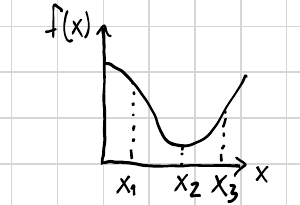
\includegraphics[width=0.32\textwidth]{figures/figura_minimo_funcion.png}

  \caption{Esquema manuscrito de una función con puntos $x_1$, $x_2$ y $x_3$.}
  \label{fig:minimum}
\end{figure}

En el punto $x_1$ de la figura \ref{fig:minimum}, la función no es mínima. Si me desplazo hacia $x_1+\delta x$ encuentro
\[
  f(x_1+\delta x)<f(x_1).
\]

Algo similar ocurre en $x_3$. Si me desplazo hacia $x_3-\delta x$ encuentro que
\[
  f(x_3-\delta x)<f(x_3),
\]
tal que $x_3$ no puede ser un mínimo.

En cambio en $x_2$ tengo un mínimo. No importa en cuál dirección me desplazo, siempre encuentro valores mayores que $f(x_2)$.

Estudiemos esos pequeños desplazamientos. Para $\delta x$ muy pequeño,
\[
  f(x+\delta x)
  \approx f(x)+f'(x)\,\delta x+\mathcal O(\delta x^2).
\]
Si queremos que $f(x+\delta x)>f(x)$ para cualquier signo de $\delta x$, necesitamos $f'(x)=0$, o también
\[
  \delta f(x)\equiv f'(x)\,\delta x=0.
\]

Hagamos lo mismo con la acción. Para encontrar el mínimo pedimos que un pequeño cambio en la trayectoria $\delta\vec q(t)$ no cambie el valor de la acción. Como fijamos condiciones de borde, consideramos sólo aquellas trayectorias que empiezan en $\vec q(t_i)$ y terminan en $\vec q(t_f)$. Entonces, para ser más precisos, pedimos que la acción sea mínima entre todas las trayectorias que van entre $\vec q(t_i)$ y $\vec q(t_f)$.

\begin{figure}
  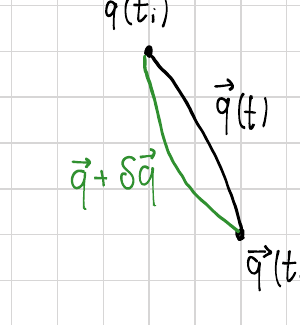
\includegraphics[width=0.28\textwidth]{figures/variacion_trayectoria.png}

  \caption{Trayectoria $\vec q(t)$ y trayectoria deformada
  $\vec q+\delta\vec q$ con extremos fijos.}
\end{figure}

Es decir, pedimos que $S$ no cambie si a la trayectoria le agregamos una deformación infinitesimal $\delta\vec q(t)$ tal que
\[
  \delta\vec q(t_i)=0,
  \qquad
  \delta\vec q(t_f)=0,
\]
y por tanto
\[
  \delta S[\vec q]=0.
\]

Partimos de
\begin{align*}
  \delta S[\vec q]
  &=S[\vec q+\delta\vec q]-S[\vec q]\\
  &=\int_{t_i}^{t_f}dt\,
  \Bigl\{
    L(\vec q+\delta\vec q,
      \dot{\vec q}+\delta\dot{\vec q},t)
    -L(\vec q,\dot{\vec q},t)
  \Bigr\}.
\end{align*}
Expandiendo a primer orden en $\delta\vec q$,
\begin{align*}
  \delta S[\vec q]
  &=\int_{t_i}^{t_f}dt\,
  \left\{
    L(\vec q,\dot{\vec q},t)
    +\frac{\partial L}{\partial q_i}\delta q_i
    +\frac{\partial L}{\partial\dot q_i}\delta\dot q_i
    -L(\vec q,\dot{\vec q},t)
  \right\}\\
  &=\int_{t_i}^{t_f}dt\,
  \left\{
    \frac{\partial L}{\partial q_i}\delta q_i
    +\frac{d}{dt}\left(
      \frac{\partial L}{\partial\dot q_i}\delta q_i
    \right)
    -\frac{d}{dt}\left(
      \frac{\partial L}{\partial\dot q_i}
    \right)\delta q_i
  \right\}.
\end{align*}
Aquí usamos
\[
  \frac{d}{dt}(fg)=\dot f\,g+f\dot g,
\]
lo que se llama integrar por partes. Entonces,
\begin{align*}
  \delta S[\vec q]
  &=\int_{t_i}^{t_f}dt\,
  \left\{
    \frac{\partial L}{\partial q_i}
    -\frac{d}{dt}\left(
      \frac{\partial L}{\partial\dot q_i}
    \right)
  \right\}\delta q_i
  +\left[
    \frac{\partial L}{\partial\dot q_i}\delta q_i
  \right]_{t_i}^{t_f}\\
  &=\int_{t_i}^{t_f}dt\,
  \left\{
    \frac{\partial L}{\partial q_i}
    -\frac{d}{dt}\left(
      \frac{\partial L}{\partial\dot q_i}
    \right)
  \right\}\delta q_i,
\end{align*}
porque usamos $\delta\vec q(t_i)=0$ y $\delta\vec q(t_f)=0$.

Pero esto tiene que ser cero para cualquier función $\delta q_i(t)$, por lo que lo que hay entre llaves tiene que ser cero.

Una cantidad que aparece con frecuencia es el \concept{momento canónico conjugado} a la variable $q_i(t)$, definido por
\[
  p_i(t)=\frac{\partial L}{\partial\dot q_i}.
\]
Para un sistema sencillo,
\[
  T=\frac12 mv^2,
  \qquad
  V=V(x),
  \qquad
  p=mv.
\]
\end{document}
